\section{Деление в формате с плавающей точкой}
\label{ch:div:fpt}

Пусть $A$ --- делимое, $d$ --- делитель. В формате с плавающей запятой эти числа будут представлены так:
\[
    A=\FloatExpression{A}{2}, d=\FloatExpression{d}{2}.
\]

Результатом деления на ненулевой делитель будет частное $q=\FloatExpression{q}{2}$:

\[
    q=\frac{A}{d}=
    \frac{\FloatExpression{A}{2}}{\FloatExpression{d}{2}}=\left(\frac{\MantissOf{A}}{\MantissOf{d}}\right)\cdot 2^{(\OrderOf{A}-\OrderOf{d})},
\]
мантисса и порядок которого будут:
\[
    \MantissOf{q} = \frac{\MantissOf{A}}{\MantissOf{d}}, \OrderOf{q}=(\OrderOf{A}-\OrderOf{d}).
\]

Мантисса частного $\MantissOf{q}$, как результат деления мантисс операндов, может оказаться ненормализованной, и в этом случае требуется её нормализовать и скорректировать порядок $\OrderOf{q}$.

\paragraph{Базовый алгоритм деления ненулевых чисел $\frac{A}{d}$.}
\begin{enumerate}
    \item Вычитанием из порядка делимого порядка делителя определяется порядок частного: $\OrderOf{q}=(\OrderOf{A}-\OrderOf{d})$. Уже на этом шаге можно выявить ошибки переполнения разрядной сетки (ПРС) или потери младших разрядов (ПМР) и завершить выполнение операции.
    \item Делением мантиссы делимого на мантиссу делителя определяется мантисса частного: $\MantissOf{q}=\frac{\MantissOf{A}}{\MantissOf{d}}$. Деление мантисс обсуждается в разделе \ref{ch:div:fpt:divmant}.
    \item Если необходимо, выполняется нормализация частного $q$. Фиксируется результат или ошибка.
\end{enumerate}

Результат деления чисел в формате с плавающей точкой редко получается точным. Как известно из обсуждения формата в главе \ref{ch:digitFormat}, абслютная погрешность представления зависит от порядка (и порой может достигать огромных величин), а относительная погрешность не превышает $\frac{100}{2^{n}}\%$, где $n$ --- разрядность двоичной мантиссы.


\subsection{Особенности деления мантисс}
\label{ch:div:fpt:divmant}

Рассмотрим пример деления двух мантисс (нормализованных дробных чисел) в десятичной системе счисления:
\[0.31136/0.25714 \approx 1.21085.\]

Как и в целочисленном делении (см. раздел \ref{ch:div:int}), цифры частного будем записывать над соответствующими разрядами делимого.

На первом шаге определяется единственная цифра целой части:
\[
    \begin{tabular}{ccccccccccc|cl}
          & 1 &,  &   &   &   &   &   &   &   &   &                     & Примечания\\ 
          \hline\hline
          & 0 &.3 & 1 & 1 & 3 & 6 &   &   &   &   & ${\div 0.25714}$    &\\
          \hline\hline
          &   &,3 & 1 & 1 & 3 & 6 &   &   &   &   &                     &\\
        - &   &,2 & 5 & 7 & 1 & 4 &   &   &   &   &                     &$=0.25714\times 1$\\
        = &   &,0 & 5 & 4 & 2 & 2 &   &   &   &   &                     &\\ \hline
    \end{tabular}
\]

На втором шаге --- первая цифра дробной части:
\[
    \begin{tabular}{ccccccccccc|cl}
          & 1 &,2 &   &   &   &   &   &   &   &   &                     & Примечания\\ 
          \hline\hline
          & 0 &.3 & 1 & 1 & 3 & 6 &   &   &   &   & ${\div 0.25714}$    &\\
          \hline\hline
          &   &,3 & 1 & 1 & 3 & 6 &   &   &   &   &                     &\\
        - &   &,2 & 5 & 7 & 1 & 4 &   &   &   &   &                     &$=0.25714\times 1$\\
        = &   &,0 & 5 & 4 & 2 & 2 &   &   &   &   &                     &\\ \hline
          &   &   &,5 & 4 & 2 & 2 &   &   &   &   &                     &\\ 
        - &   &   &,5 & 1 & 4 & 2 & 8 &   &   &   &                     &$=0.25714\times 2$\\
        = &   &   &,0 & 2 & 7 & 9 & 2 &   &   &   &                     &\\ \hline
    \end{tabular}
\]

Процесс продолжается до тех пор, пока не будет определено достаточное количество цифр результата. Все шаги процесса деления приведены на рисунке \ref{t:div:fpt:decimalDiv}.

\begin{figure}[!ht]
    \centering
    \begin{tabular}{ccccccccccc|cl}
           
          & 1 &,2 & 1 & 0 & 8 & 5 &   &   &   &   &                     & Примечания\\ 
          \hline\hline
          & 0 &.3 & 1 & 1 & 3 & 6 &   &   &   &   & ${\div 0.25714}$    &\\
          \hline\hline
          &   &,3 & 1 & 1 & 3 & 6 &   &   &   &   &                     &\\
        - &   &,2 & 5 & 7 & 1 & 4 &   &   &   &   &                     &$=0.25714\times 1$\\
        = &   &,0 & 5 & 4 & 2 & 2 &   &   &   &   &                     &\\ \hline
          &   &   &,5 & 4 & 2 & 2 &   &   &   &   &                     &\\ 
        - &   &   &,5 & 1 & 4 & 2 & 8 &   &   &   &                     &$=0.25714\times 2$\\
        = &   &   &,0 & 2 & 7 & 9 & 2 &   &   &   &                     &\\ \hline
          &   &   &   &,2 & 7 & 9 & 2 &   &   &   &                     &\\ 
        - &   &   &   &,2 & 5 & 7 & 1 & 4 &   &   &                     &$=0.25714\times 1$\\
        = &   &   &   &,0 & 2 & 2 & 0 & 6 &   &   &                     &\\ \hline
          &   &   &   &   &,2 & 2 & 0 & 6 &   &   &                     &\\ 
        - &   &   &   &   &,0 & 0 & 0 & 0 &   &   &                     &$=0.25714\times 0$\\
        = &   &   &   &   &,2 & 2 & 0 & 6 &   &   &                     &\\ \hline
          &   &   &   &   & 2 &,2 & 0 & 6 &   &   &                     &\\ 
        - &   &   &   &   & 2 &,0 & 5 & 7 & 1 & 2 &                     &$=0.25714\times 8$\\
        = &   &   &   &   & 0 &,1 & 4 & 8 & 8 & 8 &                     &\\ \hline
          &   &   &   &   &   & 1 &,4 & 8 & 8 & 8 &                     &\\ 
        - &   &   &   &   &   & 1 &,2 & 8 & 5 & 7 &                     &$=0.25714\times 5$\\
        = &   &   &   &   &   & 0 &,2 & 0 & 3 & 1 &                     &\\ \hline
    \end{tabular}
	
    \caption{$0.31136/0.25714 \approx 1.21085$ в 10СС}
    \label{t:div:fpt:decimalDiv}
\end{figure}

Схемы делительных устройств для мантисс незначительно отличаются от схемам целочисленного деления (см. рисунки \ref{t:div:int:Isp}, \ref{t:div:int:IIsp}). Схема первого способа деления мантисс приведена на рисунке \ref{t:div:fpt:Isp}, а схема второго --- на рисунке \ref{t:div:fpt:IIsp}.

\begin{figure}[!ht]
    \centering
    \begin{tabular}{c||c}
        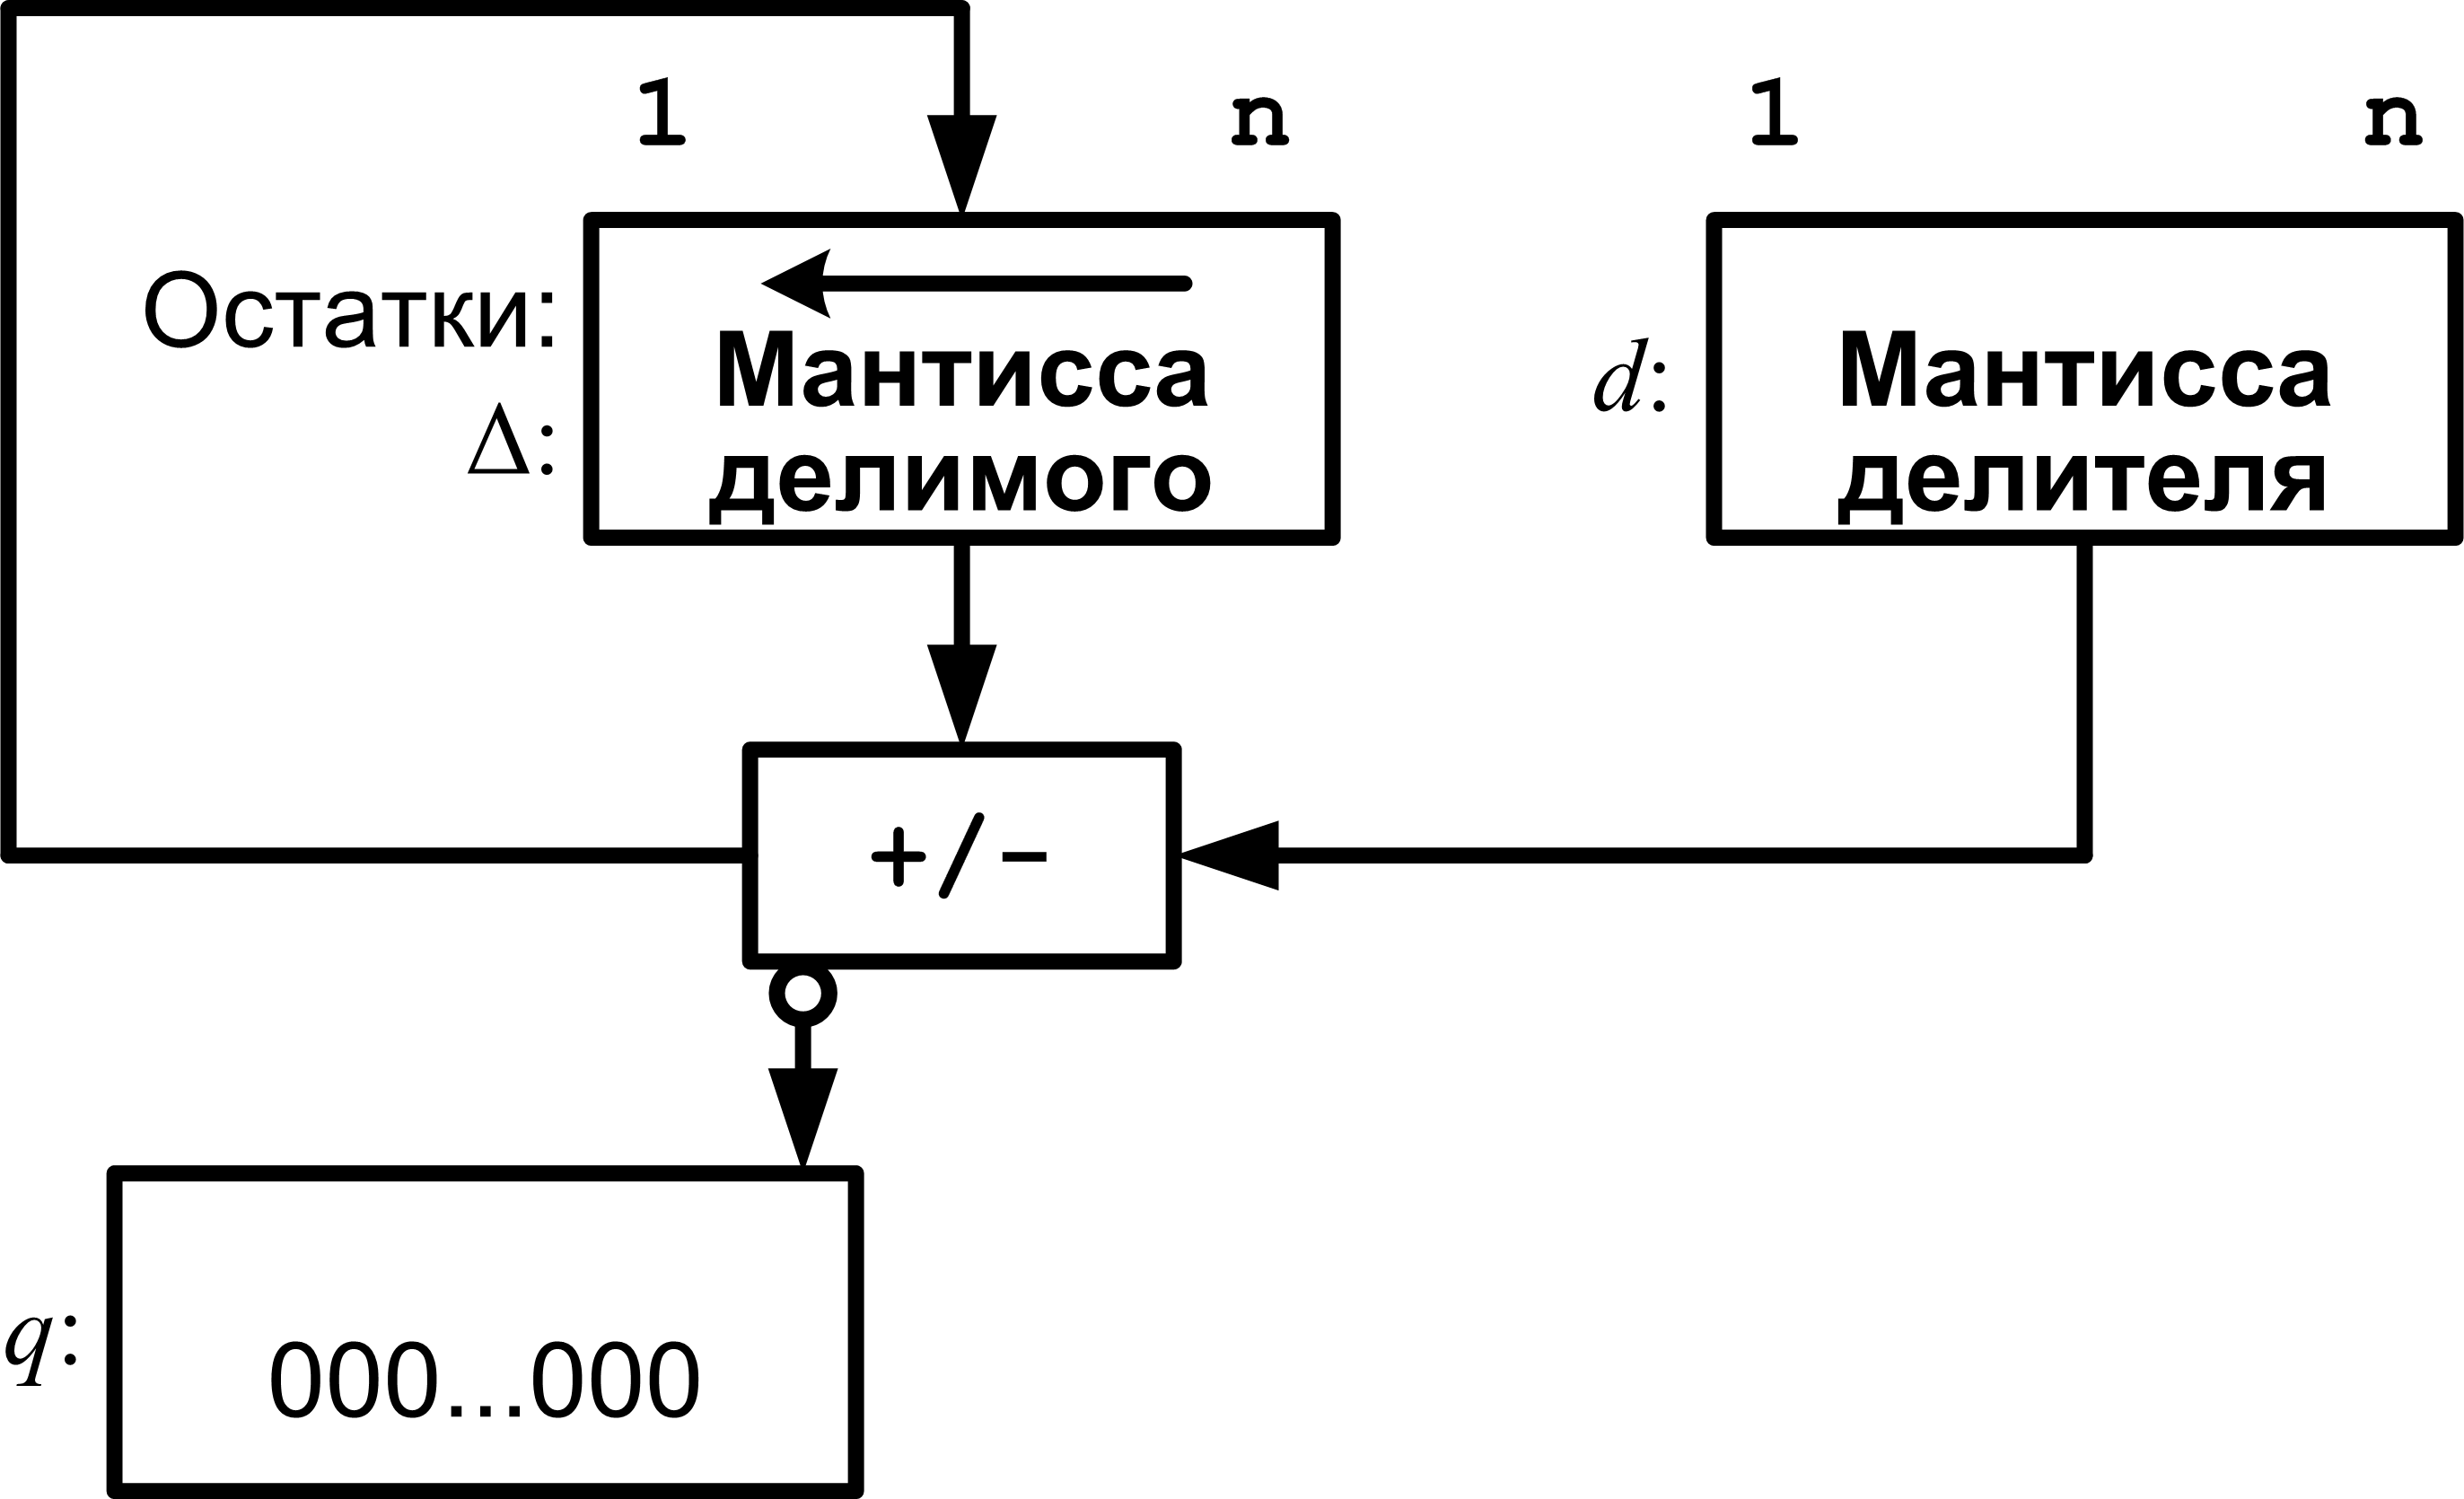
\includegraphics[width=0.47\textwidth]{fig/IFDivBegin}
            & 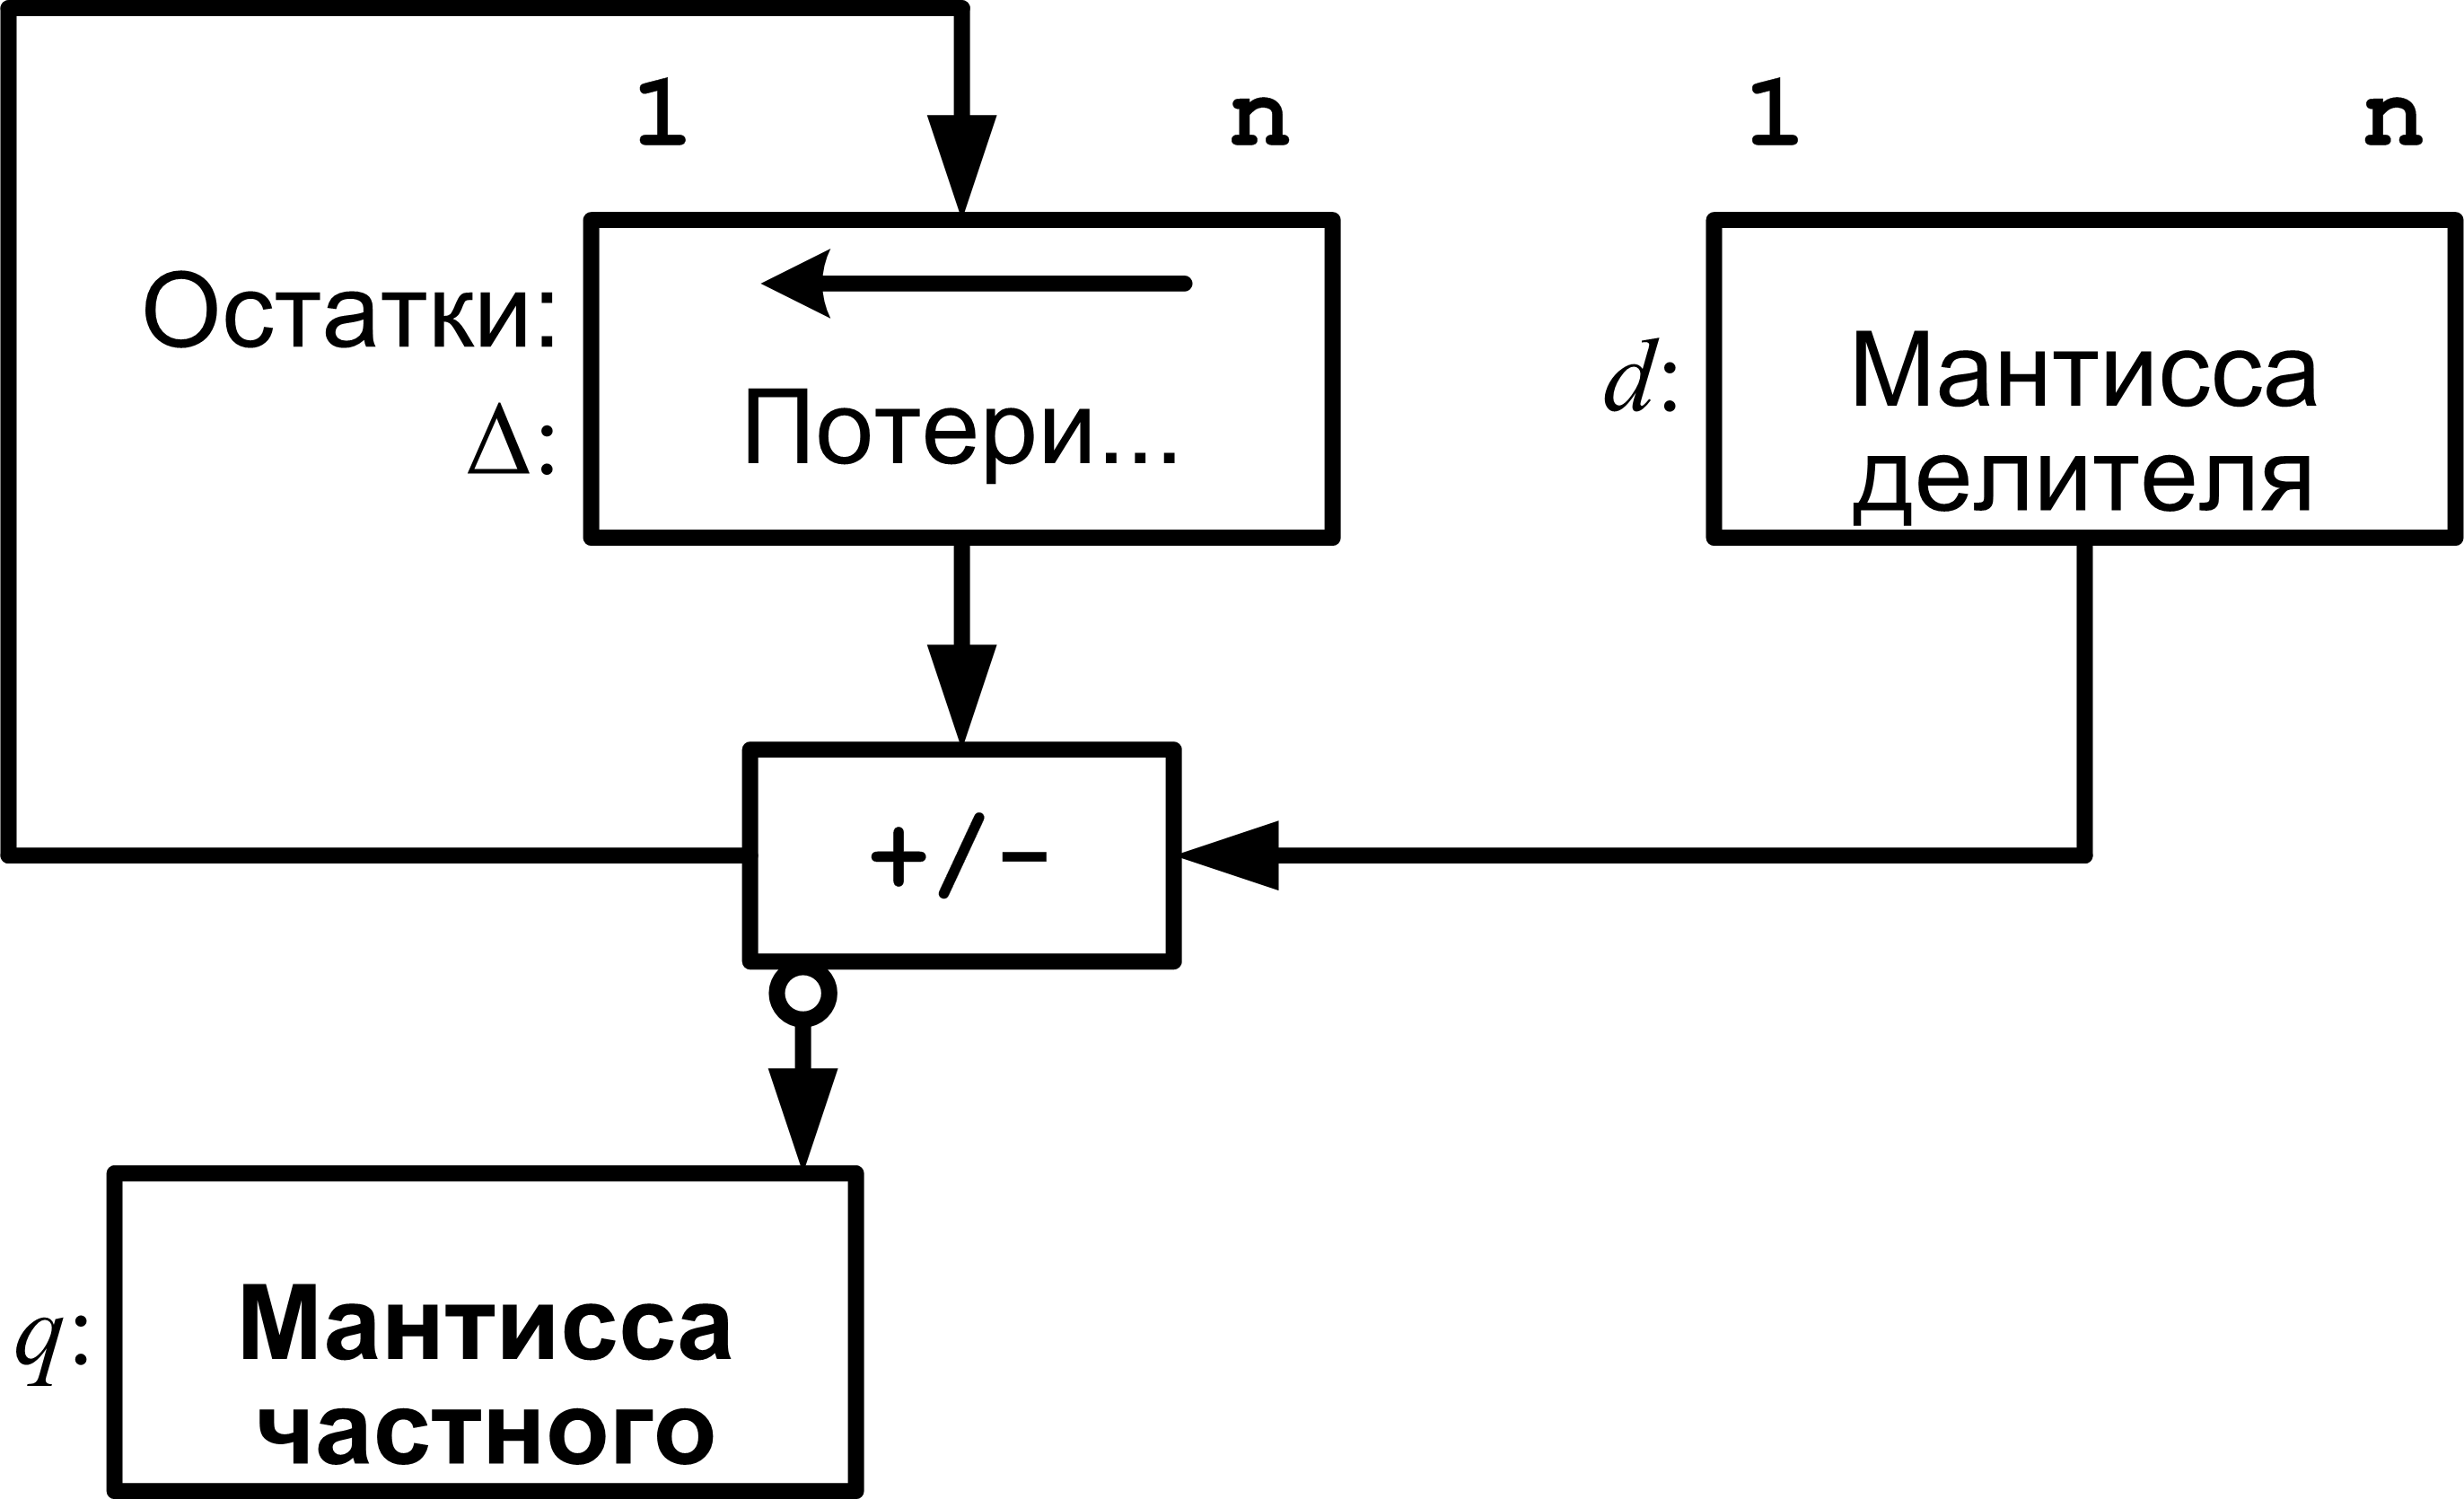
\includegraphics[width=0.47\textwidth]{fig/IFDivEnd} \\
        а) начало деления
            & б) конец деления
    \end{tabular}
    \caption{I-й способ деления нормализованных мантисс} \label{t:div:fpt:Isp}
\end{figure}

\begin{figure}[!ht]
    \centering
    \begin{tabular}{c||c}
        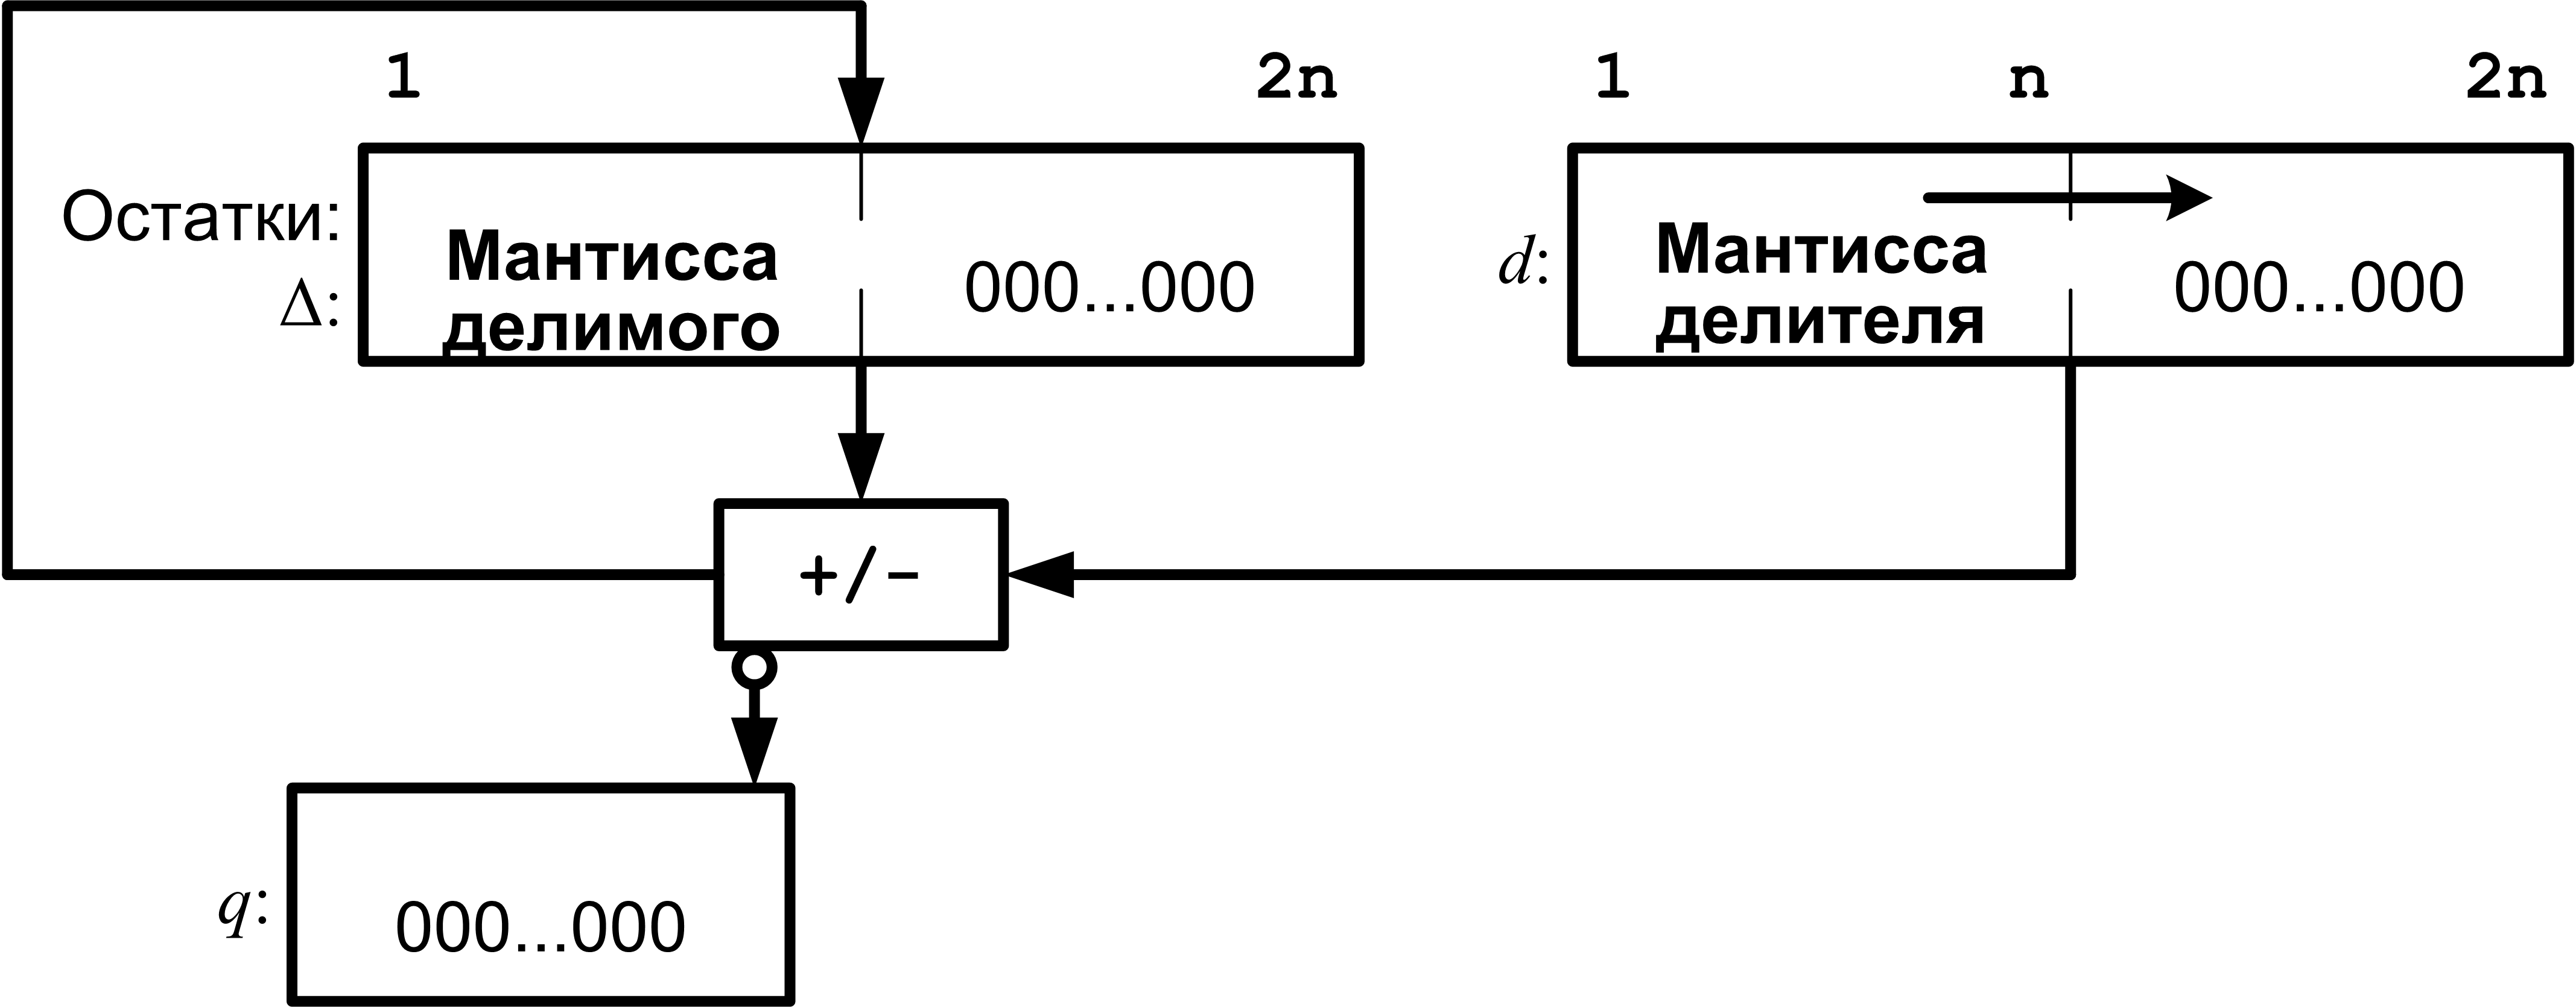
\includegraphics[width=0.47\textwidth]{fig/IIFDivBegin}
            & 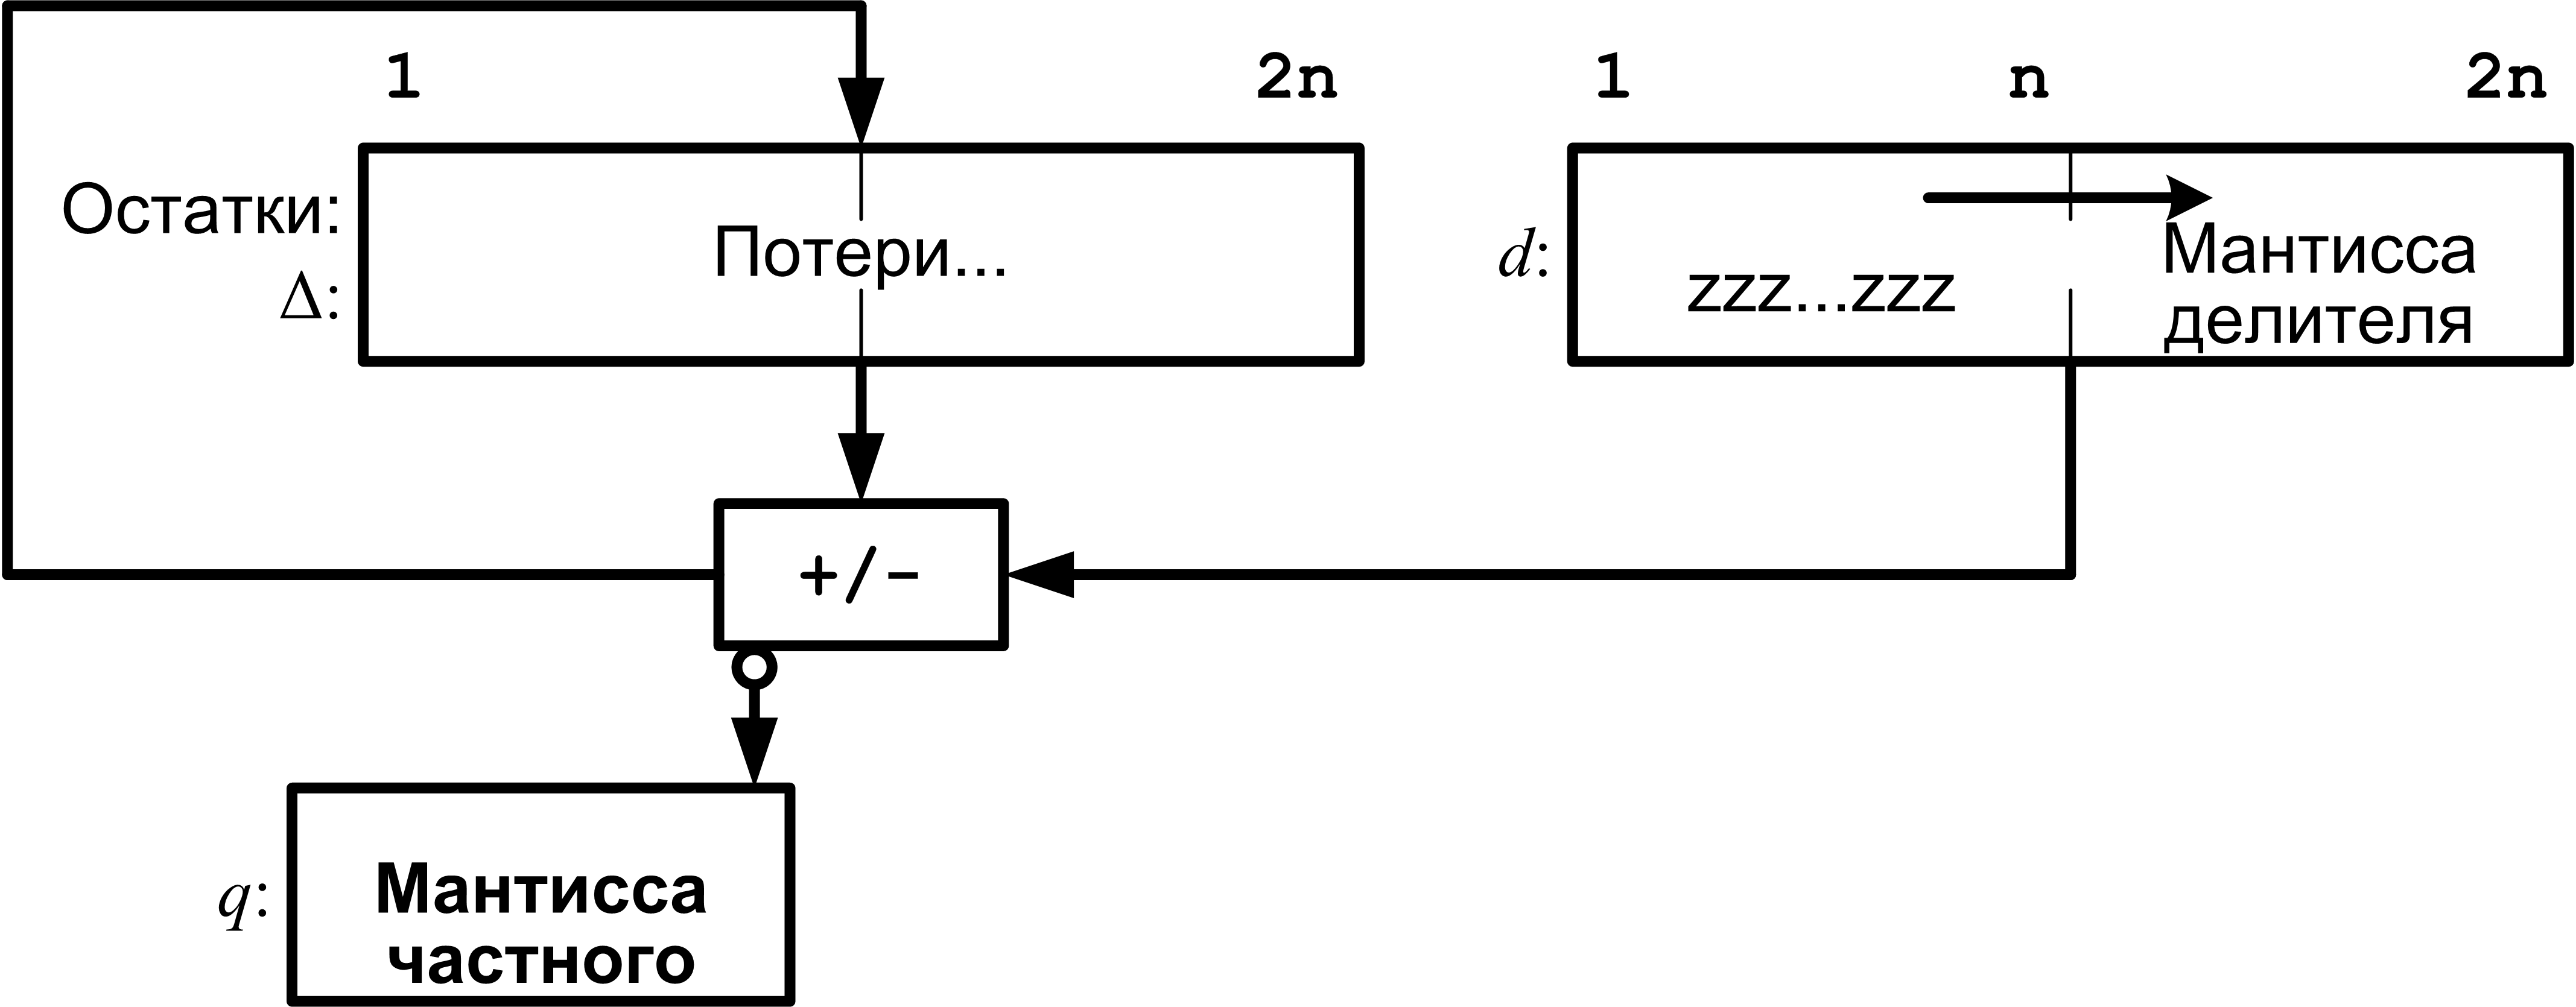
\includegraphics[width=0.47\textwidth]{fig/IIFDivEnd} \\
        а) начало деления
            & б) конец деления
    \end{tabular}
    \caption{II-й способ деления нормализованных мантисс} \label{t:div:fpt:IIsp}
\end{figure}

При делении мантисс первым способом сдвигается влево $n$-разрядный регистр остатков ($\Delta$), из значения которого в основном цикле деления вычитается значение $n$-разрядного регистра мантиссы делителя ($d$). Перед циклом деления в регистр остатков загружается делимое.

Второй способ отличается от первого тем, что регистры остатков и делителя $2n$-разрядные и сдвигается регистр делителя (вправо). В начале цикла деления мантисса делимого загружается в старшую часть регистра остатков, а делитель --- в старшую чать регистра делителя. 

Обоснование алгоритма деления мантисс без восстановления остатка аналогично обоснованию соотвествующего алгоритма для целочисленного деления. Алгоритмы с восстановлением остатка не рассматриваются, как крайне неэффективные.

Пусть формат хранит разряды модуля дробно-нормализованной мантиссы. В этом случае следует рассмотреть деление мантисс как беззнаковых дробных чисел.

Обозначим: $q$ --- частное, $\Delta$ --- остаток, $d$ --- делитель, а также соотвествующие им регистры. $A$ --- делимое.


\subsection{Деление мантисс в прямом коде}

Мантисса в прямом коде представлена знаком числа и разрядами модуля мантиссы. При этом знак и модуль мантиссы результата получаются раздельно. Знак получается сложением по <<модулю два>> (XOR) знаков операндов, а модуль мантиссы получается в результате выполнения алгоритма деления беззнаковых мантисс.

Полученный знак мантиссы в ряде случаев должен быть скорректирован, во избежание получения запрещенной в прямом коде комбинации <<отрицательного ноля>>.

\paragraph{Алгоритм деления модулей мантисс без восстановления остатков.}

\begin{enumerate}
    \item Если делитель --- ноль, фиксируется ошибка деления на ноль.
    
    \item Если делимое --- ноль, фиксируется результат: ноль.
    
    \item Вычитанием из порядка делимого порядка делителя определяется предварительный порядок частного $\OrderOf{q}\gets(\OrderOf{A}-\OrderOf{d})$. 
    
    На этом шаге может возникнуть переполнение разрядной сетки порядка. Если результат выходит за нижнюю границу представления (меньше наименьшего) то фиксируется ПМР. Ситуация ПМР может быть устранимой, когда при нормализации мантиссы увеличение порядка возвращает значение в диапазон. Если результат выходит за верхнюю границу представления (больше наибольшего), то фиксируется ПРС. Так как в процессе нормализации порядок увеличивается, то ПРС является неустранимой.
    
    \item Соотвествующим образом инициализируются регистры: остатка $\Delta$, делителя $d$, частного $q$.
    
    \item Устанавливается шаг $i\gets 0$.
    
    \item Выполняется первое вычитание делителя: $\Delta\gets(\Delta - d)$.
    
    \item Если полученный остаток $\Delta \geq 0$, то: 
    \begin{itemize}
        \item устанавливается $i\gets 1$;
        \item увеличивается на единицу предварительный порядок частного \[\OrderOf{q}\gets(\OrderOf{q} + 1);\]
        \item в младший разряд частного заносится $1$: $q_0\gets 1$.
    \end{itemize}
    
    Вследствие увеличения порядка результата может возникнуть переполнение --- в этом случае фиксируется ПРС и алгоритм завершается.
    
    \item В соответствии со схемой выполняются сдвиги регистров: $q$, $\Delta$, $d$.
    
    \item\label{fdiv:wvo:loop} Если $\Delta\ge 0$, то $\Delta\gets(\Delta - d)$, иначе $\Delta\gets(\Delta + d)$.
    
    \item Если $\Delta \ge 0$, то в младший разряд частного заносится 1, иначе --- 0. Т.е. \[q_0\gets \overline{sign(\Delta)}.\]
    
    \item Выполняется переход к следующему шагу $i\gets (i + 1)$. Если $i\geq n$, то к шагу \ref{fdiv:wvo:end}.
    
    \item В соответствии со схемой выполняются сдвиги регистров: $q$, $\Delta$, $d$ и к шагу \ref{fdiv:wvo:loop}.
    
    \item\label{fdiv:wvo:end} Определяется знак результата по знаковым разрядам операндов. Выдается результат: $\FloatExpression{q}{2}$. 
\end{enumerate}

До выдачи результата может быть выполнено округление (не обязательный, но желательный шаг).
\paragraph{Алгоритм округления.}
\begin{enumerate}
    \item Получается еще один остаток $\Delta$ (см. шаг основного алгоритма \ref{fdiv:wvo:loop}).
    
    \item Если $\Delta\ge 0$, то мантисса частного инкрементируется. Если при этом из старшего разряда мантиссы возникает перенос, то мантисса нормализуется сдвигом вправо и порядок результата увеличивается. При этом  может возникнуть ПРС порядка и вычисления завершатся ошибкой.
\end{enumerate}

\begin{Example}
    Разделить $A=-22$ на $d=9$ в формате с плавающей запятой. Для представления чисел использовать следующий формат:
    \[\FloatMyOrderX{X}{XXXXX}{X}{XXX},\]
    где в разрядах $[9:4]$ представлен прямой код мантиссы, а в разрядах $[3:0]$ --- порядок числа.
\end{Example}
\begin{Solve}
    В заданном формате числа будут представляться так:
    
    \begin{align*}
        A=-22 & \Leftrightarrow & \FloatMyOrderX{1}{10110}{0}{101}\\
          d=9 & \Leftrightarrow & \FloatMyOrderX{0}{10010}{0}{100}
    \end{align*}
    
    Предварительный порядок частного $q=\frac{A}{d}$ будет $\OrderOf{q}=5-4=1$.
    
    Деление модулей мантисс отражено в таблице \ref{t:div:fpt:IspPc}. Таблица совмещает сразу оба способа деления, так как разряды частного получаются в той же последовательности.
    
    В первом способе к регистру остатка добавлено два разряда под знак, чтобы не терять знак остатка после сдвига регистра.
    
    Во втором способе к регистрам делителя и остатка добавлен разряд справа --- это сделано только для округления, чтобы полностью избежать потерь в точности при сдвиге делителя (при отсечении добавлять разряд необязательно). 
    
    Видно, что в данном примере добавленный разряд вообще не заполняется значащим разрядом делителя. Это происходит потому, что первое вычитание делителя дает положительный остаток и потому основной цикл деления сокращается на один шаг. Если этого не сделать, то мантисса частного получится не нормализованной.
    
    Из приведенной таблицы видно, что на первом шаге получен положительный остаток, вследствие чего скорректирован порядок результата и уменьшено на единицу число шагов основного цикла деления. Таким образом выполняется нормализация результата до окончания основного цикла.
    
    \begin{figure}[!ht]
        \centering
        \begin{tabular}{c||r||r|r||l}
            \hline\hline
                & \multicolumn{1}{c||}{I-способ}
                    & \multicolumn{2}{c||}{II-способ}
                        & \\ 
            $q, \leftarrow$ 
                & \multicolumn{1}{c||}{$\Delta, \leftarrow$}
                    & \multicolumn{1}{c|}{$\Delta$}
                        & \multicolumn{1}{c||}{$d, \rightarrow$}
                            & прим.\\ 
            \hline\hline
            \Number{.....}
                & \Number{..,10110}
                    & \Number{.,10110 ..... .}
                        & \Number{.,10010 ..... .}
                            & Исх. данные.\\ \hline\hline
            \Number{....1}
                & \Addition{00,10110}
                           {11,01110}
                           {00,00100}
                    & \Addition{0,10110 ..... .}
                               {1,01110 ..... .}
                               {0,00100 00000 0}
                        & \Number{.,10010 ..... .}
                            & \Stack{$-d$; $\Delta_0>0$;}{
                                    \Stack{$\OrderOf{q}\gets(\OrderOf{q}+1)$;}{
                                        $i\gets (i+1)$;
                                    }
                              }
                              \\ \hline
            \Number{...10}
                & \Addition{00,0100.}
                           {11,01110}
                           {11,10110}
                    & \Addition{0,00100 00000 0}
                               {1,10111 0.... .}
                               {1,11011 00000 0}
                        & \Number{.,.1001 0.... .}
                            &$-d$; $\Delta_1<0$; \\ \hline
            \Number{..100}
                & \Addition{11,0110.}
                           {..,10010}
                           {11,11110}
                    & \Addition{1,11011 00000 0}
                               {.,..100 10... .}
                               {1,11111 10000 0}
                        & \Number{.,..100 10... .}
                            & $+d$; $\Delta_2<0$; \\ \hline
            \Number{.1001}
                & \Addition{11,1110.}
                           {..,10010}
                           {00,01110}
                    & \Addition{1,11111 10000 0}
                               {.,...10 010.. .}
                               {0,00001 11000 0}
                        & \Number{.,...10 010.. .}
                            & $+d$; $\Delta_3>0$; \\ \hline
            \Number{10011}
                & \Addition{00,1110.}
                           {11,01110}
                           {00,01010}
                    & \Addition{0,00001 11000 0}
                               {1,11110 1110. .}
                               {0,00000 10100 0}
                        & \Number{.,....1 0010. .}
                            & \Stack{$-d$; $\Delta_4>0$;}{
                                    Р-т отсеч.!
                              } \\ \hline\hline
            \Addition{10011}{....1}{10100}
                & \Addition{00,1010.}
                           {11,01110}
                           {00,00010}
                    & \Addition{0,00000 10100 0}
                               {1,11111 01110 .}
                               {0,00000 00010 0}
                        & \Number{.,..... 10010 .}
                            & \Stack{$-d$; $\Delta_5>0$;}{$\MantissOf{q}\gets(\MantissOf{q}+1)$;}\\ \hline
            \Number{10100}
                & 
                    &
                        &
                            & \Stack{Р-т округл.!}{$\OrderOf{q}=2$.}\\ 
        \end{tabular}
        
        \caption{Деление мантисс $\frac{-22}{9}$ I/II-сп без восстановления остатков}
        \label{t:div:fpt:IspPc}
    \end{figure}
    
    Результат с отсечением:
    \[\FloatMyOrderX{1}{10011}{0}{010}\]
    равный $-2.375$, дает абсолютную погрешность:
    \[\left|\frac{22}{9}-\frac{19}{8}\right|=\frac{5}{72}.\]
    
    Результат с округлением:
    \[\FloatMyOrderX{1}{10100}{0}{010}\]
    равный $-2.5$, дает абсолютную погрешность:
    \[\left|\frac{22}{9}-\frac{20}{8}\right|=\frac{4}{72}.\]
    
    Округление результата дает б\'{о}льшую точность.
\end{Solve}

\begin{Example}
    Разделить $A=21$ на $d=25$ в формате с плавающей точкой. Для представления чисел использовать следующий формат:
    \[\FloatMyCharX{X}{XXXXX}{XXXX},\]
    где в разрядах $[9:4]$ представлен прямой код мантиссы, а в разрядах $[3:0]$ --- характеристика (смещенный порядок) числа.
\end{Example}
\begin{Solve}
    В заданном формате числа будут представляться так:
    
    \begin{align*}
        A=21 & \Leftrightarrow & \FloatMyCharX{0}{10101}{1101}\\
        d=25 & \Leftrightarrow & \FloatMyCharX{0}{11001}{1101}
    \end{align*}
    
    Предварительная характеристика частного $q=\frac{A}{d}$ будет $\CharOf{q}=\CharOf{A}-\CharOf{d}+8=13-13+8=8$.
    
    Деление модулей мантисс отражено в таблице \ref{t:div:fpt:IspIIspPc}, совмещающей сразу оба способа деления.
    
    Из приведенной таблицы видно, что на первом шаге получен отрицательный остаток, а значит мантисса частного получается нормализованной и увеличения предварительной характеристики частного не требуется.
    
    \begin{figure}[!ht]
        \centering
        \begin{tabular}{c||r||r|r||l}
            \hline\hline
                & \multicolumn{1}{c||}{I-способ}
                    & \multicolumn{2}{c||}{II-способ}
                        & \\ 
            $q, \leftarrow$ 
                & \multicolumn{1}{c||}{$\Delta, \leftarrow$}
                    & \multicolumn{1}{c|}{$\Delta$}
                        & \multicolumn{1}{c||}{$d, \rightarrow$}
                            & прим.\\ 
            \hline\hline
            \Number{.....}
                & \Number{..,10101}
                    & \Number{.,10101 ..... .}
                        & \Number{.,11001 ..... .}
                            & Исх. данные.\\ \hline\hline
            \Number{....0}
                & \Addition{00,10101}
                           {11,00111}
                           {11,11100}
                    & \Addition{0,10101 ..... .}
                               {1,00111 ..... .}
                               {1,11100 00000 0}
                        & \Number{.,11001 ..... .}
                            &$-d$; $\Delta_0<0$; \\ \hline
            \Number{...01}
                & \Addition{11,1100.}
                           {00,11001}
                           {00,10001}
                    & \Addition{1,11100 00000 0}
                               {.,.1100 1.... .}
                               {0,01000 10000 0}
                        & \Number{.,.1100 1.... .}
                            &$+d$; $\Delta_0>0$; \\ \hline
            \Number{..011}
                & \Addition{01,0001.}
                           {11,00111}
                           {00,01001}
                    & \Addition{0,01000 10000 0}
                               {1,11001 11... .}
                               {0,00010 01000 0}
                        & \Number{.,..110 01... .}
                            &$-d$; $\Delta_1>0$; \\ \hline
            \Number{.0110}
                & \Addition{00,1001.}
                           {11,00111}
                           {11,11001}
                    & \Addition{0,00010 01000 0}
                               {1,11100 111.. .}
                               {1,11111 00100 0}
                        & \Number{.,...11 001.. .}
                            &$-d$; $\Delta_2<0$; \\ \hline
            \Number{01101}
                & \Addition{11,1001.}
                           {00,11001}
                           {00,01011}
                    & \Addition{1,11111 00100 0}
                               {.,....1 1001. .}
                               {0,00000 10110 0}
                        & \Number{.,....1 1001. .}
                            &$+d$; $\Delta_3>0$; \\ \hline
            \Number{11010}
                & \Addition{00,1011.}
                           {11,00111}
                           {11,11101}
                    & \Addition{0,00000 10110 0}
                               {1,11111 00111 .}
                               {1,11111 11101 0}
                        & \Number{.,..... 11001 .}
                            &\Stack{$-d$; $\Delta_4<0$;}{Р-т отсеч.!}\\ \hline\hline
            \Addition{11010}
                     {....1}
                     {11011}
                & \Addition{11,1101.}
                           {00,11001}
                           {00,10011}
                    & \Addition{1,11111 11101 0}
                               {.,..... .1100 1}
                               {0,00000 01001 1}
                        & \Number{.,..... .1100 1}
                            &$+d$; $\Delta_5>0$; \\ \hline
            \Number{11011}
                & 
                    & 
                        & 
                            & \Stack{Р-т округл.!}{$\CharOf{q}=8$;} 
        \end{tabular}
        
        \caption{Деление мантисс $\frac{21}{25}$ I/II-способами без восстановления остатков}
        \label{t:div:fpt:IspIIspPc}
    \end{figure}
    
    Результат с отсечением:
    \[\FloatMyCharX{0}{11010}{1000}\]
    равный $0.8125$, дает абсолютную погрешность:
    \[\left|\frac{21}{25}-\frac{26}{32}\right|=\frac{22}{800}.\]
    
    Результат с округлением:
    \[\FloatMyCharX{0}{11011}{1000}\]
    равный $0,84375$, дает абсолютную погрешность:
    \[\left|\frac{21}{25}-\frac{27}{32}\right|=\frac{3}{800}.\]
    
    Округление результата дает б\'{о}льшую точность.
\end{Solve}


\subsection{Деление мантисс в дополнительном коде}

Особенности представления чисел в формате с плавающей точкой, который использует мантиссу в дополнительном коде, отражены в примере \ref{ch:digitFormat:16DcMantChar}.

При делении мантисс желательно получить мантиссу частного сразу в дополнительном коде. Этого можно достичь, если проанализировать, что происходит с модулем остатка при вычитании делителя.
\begin{enumerate}
    \item Если после очередного действия знак остатка $\Delta$ совпадает со знаком делимого $A$, то это значит, что определяемый разряд частного $q_0$ --- единица, в противном случае --- ноль. 
    
    \[q_0\gets(sign(A)\leftrightarrow sign(\Delta))\]
    
    Здесь логическая функция тождества $(a\leftrightarrow b)$, возвращает истину, когда $(a=b)$, а функция $sign(x)$ возвращает знак числа $x$:
    \[
        sign(x)=
        \begin{cases}
            0, & x \geq 0, \\
            1, & x < 0.
        \end{cases}
    \]
    
    \item Если знаки делимого $A$ и делителя $d$ различаются, то частное $q$ должно получиться отрицательным, и в этом случае полученный в предыдущем пункте разряд $q_0$ следует инвертировать. С такой задачей прекрасно справляется функция XOR ($a\oplus b$):
    \[q_0\gets (q_0\oplus \lnot(sign(A)\leftrightarrow sign(d))).\]
    
    Строго говоря, в этом случае будет получаться обратный, а не дополнительный код частного. Далее будет показано, как, выполнив округление, можно получить правильный результат.
\end{enumerate}

Таким образом, логическое выражение для $q_0$:
\[((sign(A)\leftrightarrow sign(\Delta))\oplus \lnot(sign(A)\leftrightarrow sign(d))).\]

Используя основные тождества для функции XOR:
\begin{align*}
    (a\leftrightarrow b) & = \lnot(a\oplus b),\\
    (a\oplus b)          & = \lnot(a\leftrightarrow b),\\
    (a\oplus 0)          & = a,\\
    (a\oplus 1)          & = \lnot a,\\
    (a\oplus a)          & = 0,\\
\end{align*}
логическое выражение для $q_0$ существенно упрощается:
\begin{align*}
    ((sign(A)\leftrightarrow sign(\Delta))\oplus \lnot(sign(A)\leftrightarrow sign(d)))=\\
    =(\lnot(sign(A)\oplus sign(\Delta))\oplus (sign(A)\oplus sign(d)))=\\
    =(1\oplus sign(A) \oplus sign(\Delta) \oplus sign(A)\oplus sign(d))=\\
    =(1\oplus sign(\Delta) \oplus sign(d))=\\
    =\lnot(sign(\Delta) \oplus sign(d))=\\
    =(sign(\Delta) \leftrightarrow sign(d)).\\
\end{align*}

Таким образом, в текущий разряд частного следует записать единицу, если знак остатка совпадает со знаком делителя, и ноль --- в противном случае:
\[
    q_0\gets(sign(\Delta) \leftrightarrow sign(d)).
\]


\paragraph{Процедура поиска разряда частного.}

Вызов: $\text{ШАГ}(\Delta,d,q)$

Ввод: $\Delta$ --- значение регистра остатка, $d$ --- значение мантиссы делителя, $q$ --- значение мантиссы частного,

Вывод: $\Delta,q$ --- изменяют свое значение регистры остатка и частного.

\begin{enumerate}
    \item Если знак остатка $\Delta$ и делителя $d$ совпадают, то $\Delta\gets(\Delta-d)$, иначе $\Delta\gets(\Delta+d)$.
    \[
        \Delta\gets
            \begin{cases}
                (\Delta-d), & \text{ если $sign(\Delta)\leftrightarrow sign(d)$},\\
                (\Delta+d), & \text{ иначе}.
            \end{cases}
    \]
    
    \item Определяется значение младшего разряда мантиссы частного: $1$, если знаки остатка $\Delta$ и делителя $d$ совпадают, иначе --- $0$.
    \[
        q_0\gets(sign(\Delta) \leftrightarrow sign(d)).
    \]
    Значение подается на вход замещения младшего разряда регистра мантиссы частного $q$.
    
    \item В соответствии со схемой выполняются сдвиги регистров: $q$, $\Delta$, $d$.
\end{enumerate}


\paragraph{Алгоритм деления мантисс в дополнительном коде без восстановления остатков.}

\begin{enumerate}
    \item Если делитель --- ноль, фиксируется ошибка деления на ноль.
    
    \item Если делимое --- ноль, фиксируется результат: ноль.
    
    \item Вычитанием из порядка делимого порядка делителя определяется предварительный порядок частного $\OrderOf{q}\gets(\OrderOf{A}-\OrderOf{d})$.
    
    На этом шаге может возникнуть ситуации ПМР (как устранимого, так и неустранимого) и неустранимого ПРС.
    
    \item \label{fdiv:dc:init} Соотвествующим образом инициализируются регистры остатка $\Delta$ и делителя $d$. Младший разряд регистра частного $q_0$ заполняются знаком будущего результата: $q_0\gets (sign(A)\oplus sign(d))$.

    \item Устанавливается шаг $i\gets 1$.
    
    \item \label{fdiv:dc:loop} Выполняется процедура поиска разряда частного:
    \[
        \text{ШАГ}(\Delta,d,q).
    \]
    
    \item $i\gets (i + 1)$. Если $i < n$, то выполняется переход к пункту \ref{fdiv:dc:loop}.
    
    \item В основном цикле были определены $(n-1)$ разрядов мантиссы частного. Старший (знаковый) разряд мантиссы частного был определен на шаге \ref{fdiv:dc:init}.
    
    \item Если на данном этапе старшая пара разрядов мантиссы имеет значения \Machine{01} или \Machine{10} (то есть мантисса оказалась нормализованной), то предварительный порядок частного следует увеличить на единицу $\OrderOf{q}\gets(\OrderOf{q} + 1)$ и выполнить переход к шагу \ref{fdiv:dc:end}. При увеличении порядка может возникнуть ситуация ПРС.
    
    \item Иначе, если старшая пара разрядов мантиссы имеет значения \Machine{00} или \Machine{11}, то следует выполнить еще один шаг основного цикла, чтобы определить очередной разряд мантиссы частного:
    \[
        \text{ШАГ}(\Delta,d,q).
    \]

    На этом шаге коррекции порядка $\OrderOf{q}$ не требуется, а мантисса после сделанного шага должна нормализоваться автоматически.
    
    \item \label{fdiv:dc:end} Фиксируется ошибка или выдается результат: $\FloatExpression{q}{2}$. 
    
    Мантисса частного на данном шаге, строго говоря, получается в обратном коде, но при большой разрядности разница (погрешность) оказывается невелика. Чтобы уменьшить погрешность вычислений, можно выполнить округление.
\end{enumerate}

Если снять ограничение на количество шагов в данном алгоритме и ограничения размерности регистров схемы деления, то технически можно получить сколь угодно много разрядов мантиссы частного. Пусть разрядность мантиссы $n$-бит и требуется грамотно выполнить округление:

\[
    .\underbrace{\overbrace{xx\cdots xx}^{\MantissOf{q}}}_n xx\cdots
\]

Обобщенно, результаты деления могут быть следующими (см. также особенности округления дополнительных кодов в разделе \ref{ch::float::ss::round}).
\begin{itemize}
    \item В случае положительного результата
    \[.\overbrace{0x\cdots xx}^{\MantissOf{q}} xx\cdots\]
    достаточно рассмотреть следующие случаи:
    
    \begin{itemize}
        \item $.\overbrace{0x\cdots xx}^{\MantissOf{q}} 0x\cdots$.
        
        Отбрасываемая часть начинается с нуля. В этом случае поправок не требуется.

        \item $.\overbrace{0x\cdots xx}^{\MantissOf{q}} 1x\cdots$.
        
        В этом случае требуется поправка $\MantissOf{q}\gets(\MantissOf{q}+1)$.
    \end{itemize}
    
    \item В случае отрицательного результата
    \[.\overbrace{1x\cdots xx}^{\MantissOf{q}} xx\cdots\]
    следует рассмотреть следующие случаи:
    
    \begin{itemize}
        \item $.\overbrace{1x\cdots xx}^{\MantissOf{q}} 00\cdots 0\cdots$.
        
        В отбрасываемой части нули. Ситуация возникает при делении на положительный делитель, а на $i$-м шаге основного цикла получается нулевой остаток. Результат получен в дополнительном коде и поправок не требует.
        
        \item $.\overbrace{1x\cdots xx}^{\MantissOf{q}} 0x\cdots x1x\cdots$.
        
        Старший разряд отбрасываемой части --- нуль, а за ним следует произвольная последовательность, в которой встречаются и единицы и нули. В этом случае отбрасываемая часть модуля мантиссы начинается с единицы и требуется получить:
        \[
            -(\overline{\MantissOf{q}}+1)=-(-\MantissOf{q}-1+1)=\MantissOf{q}.
        \]
        
        Поправок не требуется.
        
        \item $.\overbrace{1x\cdots xx}^{\MantissOf{q}} 10\cdots 0\cdots$.
        
        Старший разряд отбрасываемой части --- 1, а все последующие разряды --- нули. Такая комбинация разрядов на выходе не возникнет.

        \item $.\overbrace{1x\cdots xx}^{\MantissOf{q}} 11\cdots 1\cdots$.
        
        В отбрасываемой части все единицы. Такая ситуация возникает, когда выполняется деление на отрицательный делитель и на $i$-м шаге основного цикла в остатке образуется ноль. 
        
        В этом случае требуется поправка $\MantissOf{q}\gets(\MantissOf{q}+1)$.
        
        \item $.\overbrace{1x\cdots xx}^{\MantissOf{q}} 1x\cdots x1x\cdots$.
        
        В старшем разряде отбрасываемой части --- 1, далее следет произвольная последовательность в которой встречаются и единицы и нули. В этом случае отбрасываемая часть модуля мантиссы начинается с нуля и требуется получить:
        \[-(\overline{\MantissOf{q}})=-(-\MantissOf{q}-1)=(\MantissOf{q}+1).\]
        
        Требуется поправка: $\MantissOf{q}\gets(\MantissOf{q}+1)$.
        
    \end{itemize}
\end{itemize}

\begin{Rule}
    Если отбрасываемая часть начинается с единицы, то мантиссу округляемого частного следует увеличить на единицу.
\end{Rule}


\paragraph{Алгоритм округления.}
\begin{enumerate}
    \item Выполняется поиск старшего разряда отбрасываемой части. Для этого можно выполнить процедуру поиска разряда частного:
    \[
        \text{ШАГ}(\Delta,d,q),
    \]
    но не выполнять сдвиг регистра частного.
    
    \item Если найденный старший разряд отбрасываемой части --- ноль, то алгоритм завершается, коррекции мантиссы не требуется.
    
    \item В противном случае мантисса результата увеличивается на единицу. Это действие может повлечь одно из следующих взаимоисключающих последствий.
    \begin{itemize}
        \item Если мантисса до округления была положительной, то после инкремента может возникнуть временное ПРС мантиссы. Для коррекции мантисса сдвигается вправо, а порядок увеличивается на единицу. Возможно ПРС.
        
        \item Если мантисса до округления была отрицательной, то после инкремента может наступить потеря нормализации. Для коррекции мантисса сдвигается влево, а порядок на единицу уменьшается. Возможно ПМР.
        
        \item Ни ПРС мантиссы, ни потери нормализации не возникнет. Никаких действий по коррекции не требуется.
    \end{itemize}
\end{enumerate}

\begin{Example}
    Разделить $A=-23$ на $d=19$ в формате с плавающей запятой. Для представления чисел использовать следующий формат:
    \[\FloatMyDcOrderX{XXXXXX}{X}{XXX},\]
    где в разрядах $[9:4]$ представлен дополнительный код мантиссы, а в разрядах $[3:0]$ --- порядок числа.
\end{Example}
\begin{Solve}
    В заданном формате числа будут представляться так (см. особенности представления в примере \ref{ch:digitFormat:16DcMantChar}):
    
    \begin{align*}
        A=-23 & \Leftrightarrow & \FloatMyDcOrderX{101001}{0}{101}\\
         d=19 & \Leftrightarrow & \FloatMyDcOrderX{010011}{0}{101}
    \end{align*}
    
    Предварительный порядок частного $q=\frac{A}{d}$ будет $\OrderOf{q}=5-5=0$.
    
    Деление модулей мантисс отражено в таблице \ref{t:div:fpt:DcRounding}.
    
    В первом способе к регистру остатка добавлен разряд под знак, чтобы не терять знак остатка после сдвига регистра.
    
    Во втором способе к регистрам делителя и остатка добавлен разряд справа --- это сделано только для округления, чтобы полностью избежать потерь в точности при сдвиге делителя. Видно, что в данном примере добавленный разряд вовсе не заполняется значащим разрядом делителя --- это происходит из-за того, что после $(n-1)$ шагов основного цикла, выполняются условия нормализации мантиссы и поэтому не выполняется поиск $n$-го разряда частного.

    Из приведенной таблицы видно, что уже на $5$-м шаге цикла мантисса оказалась нормализованной. Такая ситуация означает, что результат получается <<с целой частью>>, и поэтому предварительный порядок $\OrderOf{q}$ увеличивается на единицу.
    
    \begin{figure}[!ht]
        \centering
        \begin{tabular}{c||r||r|r||l}
            \hline\hline
                & \multicolumn{1}{c||}{I-способ}
                    & \multicolumn{2}{c||}{II-способ}
                        & \\ 
            $q, \leftarrow$ 
                & \multicolumn{1}{c||}{$\Delta, \leftarrow$}
                    & \multicolumn{1}{c|}{$\Delta$}
                        & \multicolumn{1}{c||}{$d, \rightarrow$}
                            & прим.\\ 
            \hline\hline
            \Number{.,....1}
                & \Number{11,01001}
                    & \Number{1,01001 ..... .}
                        & \Number{.,10011 ..... .}
                            & Исх. данные.\\ \hline\hline
            \Number{.,...10}
                & \Addition{11,01001}
                           {..,10011}
                           {11,11100}
                    & \Addition{1,01001 ..... .}
                               {.,10011 ..... .}
                               {1,11100 00000 0}
                        & \Number{.,10011 ..... .}
                            & \Stack{$+d$;}{$s(\Delta_1)\not= s(d)$;}
                              \\ \hline
            \Number{.,..101}
                & \Addition{11,1100.}
                           {..,10011}
                           {00,01011}
                    & \Addition{1,11100 00000 0}
                               {.,.1001 1.... .}
                               {0,00101 10000 0}
                        & \Number{.,.1001 1.... .}
                            &\Stack{$+d$;}{$s(\Delta_2)= s(d)$;} \\ \hline
            \Number{.,.1011}
                & \Addition{00,1011.}
                           {11,01101}
                           {00,00011}
                    & \Addition{0,00101 10000 0}
                               {1,11011 01... .}
                               {0,00000 11000 0}
                        & \Number{.,..100 11... .}
                            & \Stack{$-d$;}{$s(\Delta_3)= s(d)$;} \\ \hline
            \Number{.,10110}
                & \Addition{00,0011.}
                           {11,01101}
                           {11,10011}
                    & \Addition{0,00000 11000 0}
                               {1,11101 101.. .}
                               {1,11110 01100 0}
                        & \Number{.,...10 011.. .}
                            & \Stack{$-d$;}{$s(\Delta_4)\not= s(d)$;} \\ \hline
            \Number{1,01100}
                & \Addition{11,0011.}
                           {..,10011}
                           {11,11001}
                    & \Addition{1,11110 01100 0}
                               {.,....1 0011. .}
                               {1,11111 10010 0}
                        & \Number{.,....1 0011. .}
                            & \StackFour{$+d$;}
                                        {$s(\Delta_5)\not= s(d)$;}
                                        {$\OrderOf{q}\gets(\OrderOf{q} + 1)$}
                                        {Р-т отсеч.!}
                                \\ \hline\hline
            \Addition{1,01100}{.,....1}{1,01101}
                & \Addition{11,1001.}
                           {00,10011}
                           {00,00010}
                    & \Addition{1,11111 10010 0}
                               {.,..... 10011 .}
                               {0,00000 00101 0}
                        & \Number{.,..... 10011 .}
                            & \StackThree{$+d$;}
                                         {$s(\Delta_6)= s(d)$;}
                                         {$\MantissOf{q}\gets(\MantissOf{q}+1)$;}\\ \hline
            \Number{1,01101}
                & 
                    &
                        &
                            & \Stack{Р-т округл.!}{$\OrderOf{q}=1$.}\\ 
        \end{tabular}
        
        \caption{Деление мантисс $\frac{-23}{19}$ в дополнительном коде I/II-сп без восстановления остатков}
        \label{t:div:fpt:DcRounding}
    \end{figure}
    
    Результат с отсечением:
    \[\FloatMyDcOrderX{101100}{0}{001}\]
    равный $-1.25$, дает абсолютную погрешность:
    \[\left|\frac{23}{19}-\frac{20}{16}\right|=\frac{12}{304}.\]
    
    Результат с округлением:
    \[\FloatMyDcOrderX{101101}{0}{001}\]
    равный $-1.1875$, дает абсолютную погрешность:
    \[\left|\frac{23}{19}-\frac{19}{16}\right|=\frac{7}{304}.\]
    
    Округление в дополнительном коде позволяет получать результат с меньшей погрешностью, а также без погрешности в случае <<деления нацело>>, когда на некотором шаге основного цикла деления получается нулевой остаток.
\end{Solve}

\begin{Example}
    Разделить $A=21$ на $d=-25$ в формате с плавающей запятой. Для представления чисел использовать следующий формат:
    \[\FloatMyDcCharX{XXXXXX}{XXXX},\]
    где в разрядах $[9:4]$ представлен дополнительный код мантиссы, а в разрядах $[3:0]$ --- характеристика числа.
\end{Example}
\begin{Solve}
    В заданном формате числа будут представляться так (см. особенности представления в примере \ref{ch:digitFormat:16DcMantChar}):
    
    \begin{align*}
        A=21  & \Leftrightarrow & \FloatMyDcCharX{010101}{1101}\\
        d=-25 & \Leftrightarrow & \FloatMyDcCharX{100111}{1101}
    \end{align*}
    
    Предварительная характеристика частного $q=\frac{A}{d}$ будет $\CharOf{q}=13-13+8=0$.
    
    Деление модулей мантисс отражено в таблице \ref{t:div:fpt:DcUnRounding}.
    
    Из приведенной таблицы видно, что на $5$-м шаге цикла мантисса оказалась ненормализованной поэтому выполняется процедура поиска разряда частного и на $6$-м шаге процесс завершается автоматической нормализацией мантиссы.
    
    \begin{figure}[!ht]
        \centering
        \begin{tabular}{c||r||r|r||l}
            \hline\hline
                & \multicolumn{1}{c||}{I-способ}
                    & \multicolumn{2}{c||}{II-способ}
                        & \\ 
            $q, \leftarrow$ 
                & \multicolumn{1}{c||}{$\Delta, \leftarrow$}
                    & \multicolumn{1}{c|}{$\Delta$}
                        & \multicolumn{1}{c||}{$d, \rightarrow$}
                            & прим.\\ 
            \hline\hline
            \Number{.,....1}
                & \Number{00,10101}
                    & \Number{0,10101 ..... .}
                        & \Number{1,00111 ..... .}
                            & Исх. данные.\\ \hline\hline
            \Number{.,...11}
                & \Addition{00,10101}
                           {11,00111}
                           {11,11100}
                    & \Addition{0,10101 ..... .}
                               {1,00111 ..... .}
                               {1,11100 00000 0}
                        & \Number{1,00111 ..... .}
                            & \Stack{$+d$;}{$s(\Delta_1)= s(d)$;}
                              \\ \hline
            \Number{.,..110}
                & \Addition{11,1100.}
                           {00,11001}
                           {00,10001}
                    & \Addition{1,11100 00000 0}
                               {.,.1100 1.... .}
                               {0,01000 10000 0}
                        & \Number{1,10011 1.... .}
                            &\Stack{$-d$;}{$s(\Delta_2)\not= s(d)$;} \\ \hline
            \Number{.,.1100}
                & \Addition{01,0001.}
                           {11,00111}
                           {00,01001}
                    & \Addition{0,01000 10000 0}
                               {1,11001 11... .}
                               {0,00010 01000 0}
                        & \Number{1,11001 11... .}
                            & \Stack{$+d$;}{$s(\Delta_3)\not= s(d)$;} \\ \hline
            \Number{.,11001}
                & \Addition{00,1001.}
                           {11,00111}
                           {11,11001}
                    & \Addition{0,00010 01000 0}
                               {1,11100 111.. .}
                               {1,11111 00100 0}
                        & \Number{1,11100 111.. .}
                            & \Stack{$+d$;}{$s(\Delta_4)= s(d)$;} \\ \hline
            \Number{1,10010}
                & \Addition{11,1001.}
                           {00,11001}
                           {00,01011}
                    & \Addition{1,11111 00100 0}
                               {.,....1 1001. .}
                               {0,00000 10110 0}
                        & \Number{1,11110 0111. .}
                            & \StackThree{$-d$;}
                                        {$s(\Delta_5)\not= s(d)$;}
                                        {Ещё шаг!}
                                \\ \hline
            \Number{1,00101}
                & \Addition{00,1011.}
                           {11,00111}
                           {11,11101}
                    & \Addition{0,00000 10110 0}
                               {1,11111 00111 .}
                               {1,11111 11101 0}
                        & \Number{1,11111 00111 .}
                            & \StackThree{$+d$;}
                                        {$s(\Delta_6)= s(d)$;}
                                        {Р-т отсеч.!}
                                \\ \hline\hline
            \Addition{1,00101}{.,....0}{1,00101}
                & \Addition{11,1101.}
                           {00,11001}
                           {00,10011}
                    & \Addition{1,11111 11101 0}
                               {0,00000 01100 1}
                               {0,00000 01001 1}
                        & \Number{1,11111 10011 1}
                            & \Stack{$-d$;}
                                    {$s(\Delta_7)\not= s(d)$;}
                                \\ \hline
            \Number{1,00101}
                & 
                    &
                        &
                            & \Stack{Р-т округл.!}{$\CharOf{q}=8$.}\\ 
        \end{tabular}
        
        \caption{Деление мантисс $\frac{21}{-25}$ в дополнительном коде I/II-сп без восстановления остатков}
        \label{t:div:fpt:DcUnRounding}
    \end{figure}
    
    Результат с отсечением совпадает с округленным результатом:
    \[\FloatMyDcCharX{100101}{1000}\]
    равный $-0.84375$, дает абсолютную погрешность:
    \[\left|\frac{21}{-25}-\frac{-27}{32}\right|=\frac{3}{800}.\]
    
    Непосредственной проверкой можно убедиться, что ближайшие варианты с той же характеристикой:
    \begin{align*}
        \FloatMyDcCharX{100100}{1000}\\
        \FloatMyDcCharX{100110}{1000}
    \end{align*}
    дают б\'{о}льшую погрешность.
\end{Solve}


\subsection{Исходы операции деления}

%Исходы в формате с плавающей запятой --- обсудить отдельно в формате с плавающей запятой.

ПРС, возникает, когда результат вычитания порядков операндов выходит за пределы представления \emph{положительных} порядков. При делении ситуация ПРС является неустранимой, так как в процессе нормализации порядок результата может только увеличиваться. В случае ПРС фиксируется ошибка вычислений.

ПМР, возникает, когда результат вычитания порядков операндов выходит за пределы представления \emph{отрицательных} порядков. При делении ситуация ПМР может оказаться устранимой, так как в процессе нормализации порядок результата может увеличиваться и порядок результата при этом может <<вернуться>> в диапазон. В случае ПМР --- в качестве результата выдается ноль и фиксируется ситуация ПМР (например, устанавливается соотвествущий флаг).
